Over 27 days Silver has 3{,}485{,}540 stop calls (153k on a weekday, 55k on a Sunday). 55\% of
measured stops are on time and 0.18\% are cancelled. The afternoon rush is the worst: on
weekdays only 33\% of stops at 15:00 are on time, and the morning rush (7--8) is at about 48\%
(Figure~\ref{fig:heatmap}). Weekends are better than weekdays (62\% against 54\%).

X39 is the worst line with 14\% on time (Figure~\ref{fig:lines}). It is an express line from
Stavanger via UiS and Forus to Ålgård. Morning trips are already almost 5 minutes late at the
first stop and about 16 minutes late at the last. Four of the ten worst lines are school routes
(\code{SK}). X39 and the school routes run mostly in the rush hours, when traffic is heaviest,
which fits the heatmap. Three of the ten are night lines (\code{N}).

\begin{figure}[htb]
\centering
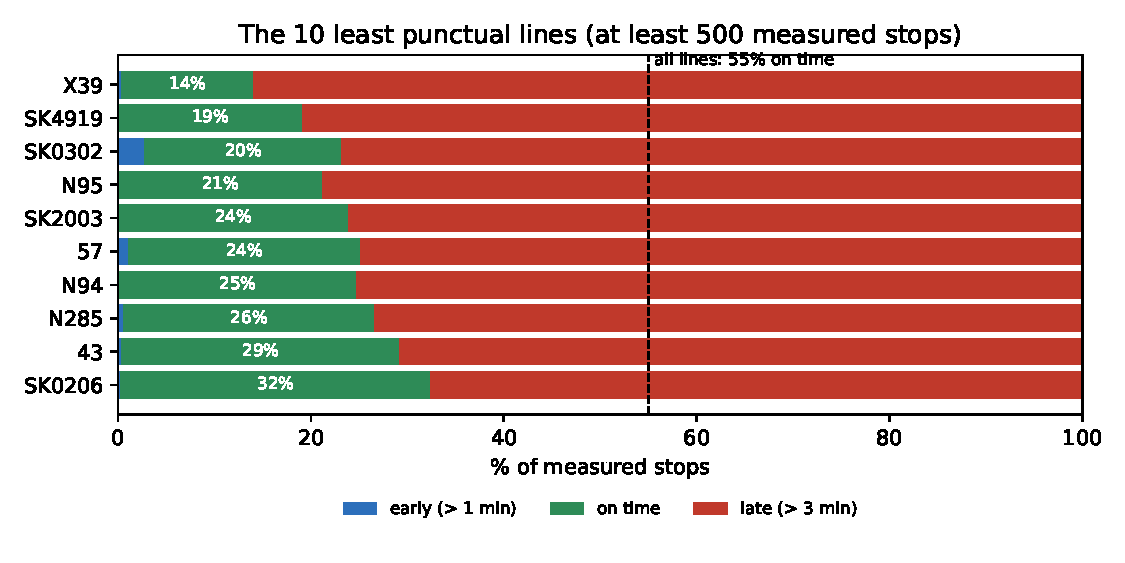
\includegraphics[width=\linewidth]{2_worst_lines.pdf}
\caption{The ten least punctual lines (at least 500 measured stops).}
\label{fig:lines}
\end{figure}
